\begin{frame}[fragile, shrink=50]
  \frametitle{Computational hemodynamics (contd.)}

  \vspace{2cm}

  \begin{columns}

    \begin{column}{0.5\textwidth}
      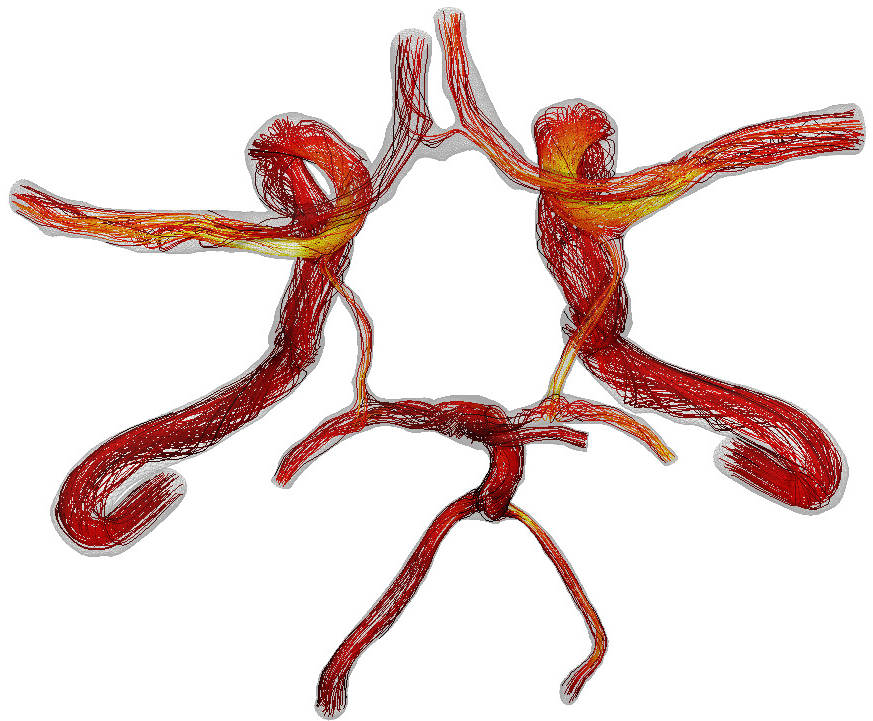
\includegraphics[width=\textwidth]{png/circle_of_willis_simulation.png}
    \end{column}

    \begin{column}{0.5\textwidth}
      \begin{python}
# Define Cauchy stress tensor
def sigma(v,w):
    return 2.0*mu*0.5*(grad(v) + grad(v).T)  - w*Identity(v.cell().d)

# Define symmetric gradient
def epsilon(v):
    return  0.5*(grad(v) + grad(v).T)

# Tentative velocity step (sigma formulation)
U = 0.5*(u0 + u)
F1 = rho*(1/k)*inner(v, u - u0)*dx + rho*inner(v, grad(u0)*(u0 - w))*dx \
   + inner(epsilon(v), sigma(U, p0))*dx \
   + inner(v, p0*n)*ds - mu*inner(grad(U).T*n, v)*ds \
   - inner(v, f)*dx
a1 = lhs(F1)
L1 = rhs(F1)

# Pressure correction
a2 = inner(grad(q), k*grad(p))*dx
L2 = inner(grad(q), k*grad(p0))*dx - q*div(u1)*dx

# Velocity correction
a3 = inner(v, u)*dx
L3 = inner(v, u1)*dx + inner(v, k*grad(p0 - p1))*dx
      \end{python}
    \end{column}

  \end{columns}

  % Compensate for scaling
  \huge

  \vspace{0.5cm}

  \begin{itemize}
  \item
    The Navier--Stokes solver is implemented in Python/FEniCS
  \item
    FEniCS allows solvers to be implemented in a minimal amount of code
  \end{itemize}

  \reference{Valen-Sendstad, Mardal, Logg}
            {Computational hemodynamics}
            {2011}

\end{frame}
